\ifx\PREAMBLE\undefined
\documentclass{report}
\usepackage[format = hang, font = bf]{caption}
% The following is needed in order to make the code compatible
% with both latex/dvips and pdflatex. Added for using UML generated by MetaUML.
\ifx\pdftexversion\undefined
\usepackage[dvips]{graphicx}
\else
\usepackage[pdftex]{graphicx}
\DeclareGraphicsRule{*}{mps}{*}{}
\fi
\usepackage{array}
\usepackage{amsmath}
\usepackage{amsthm}
\usepackage{mathtools}
\usepackage{boxedminipage}
\usepackage{listings}
\usepackage{makecell}%diagonal line in table
\usepackage{float}%allowing forceful figure[H]
\usepackage{xcolor}
\usepackage{amsfonts}%allowing \mathbb{R}
\usepackage{amssymb}
\usepackage{alltt}
\usepackage{algorithmicx}
\usepackage[chapter]{algorithm} 
%chapter option ensures that algorithms are numbered within each chapter rather than in the whole article
\usepackage[noend]{algpseudocode} %If end if, end procdeure, etc is expected to appear, remove the noend option
\usepackage{xspace}
\usepackage{color}
\usepackage{url}
\def\UrlBreaks{\do\A\do\B\do\C\do\D\do\E\do\F\do\G\do\H\do\I\do\J\do\K\do\L\do\M\do\N\do\O\do\P\do\Q\do\R\do\S\do\T\do\U\do\V\do\W\do\X\do\Y\do\Z\do\[\do\\\do\]\do\^\do\_\do\`\do\a\do\b\do\c\do\d\do\e\do\f\do\g\do\h\do\i\do\j\do\k\do\l\do\m\do\n\do\o\do\p\do\q\do\r\do\s\do\t\do\u\do\v\do\w\do\x\do\y\do\z\do\0\do\1\do\2\do\3\do\4\do\5\do\6\do\7\do\8\do\9\do\.\do\@\do\\\do\/\do\!\do\_\do\|\do\;\do\>\do\]\do\)\do\,\do\?\do\'\do+\do\=\do\#\do\-}
\usepackage[breaklinks = true]{hyperref}
\lstset{
language = C++, 
showspaces = false,
breaklines = true, 
tabsize = 2, 
numbers = left, 
extendedchars = false, 
basicstyle = {\ttfamily \footnotesize}, 
keywordstyle=\color{blue!70}, 
commentstyle=\color{gray}, 
frame=shadowbox, 
rulesepcolor=\color{red!20!green!20!blue!20}, 
numberstyle={\color[RGB]{0,192,192}}, 
moredelim=[is][\underbar]{_}{_}
}
\mathchardef\myhyphen="2D
% switch-case environment definitions
\algblock{switch}{endswitch} 
\algblock{case}{endcase}
%\algrenewtext{endswitch}{\textbf{end switch}} %If end switch is expected to appear, uncomment this line.
\algtext*{endswitch} % Make end switch disappear
\algtext*{endcase}
\algnewcommand\algorithmicinput{\textbf{input:}}
\algnewcommand\Input{\item[\algorithmicinput]}
\algnewcommand\algorithmicoutput{\textbf{output:}}
\algnewcommand\Output{\item[\algorithmicoutput]}
\allowdisplaybreaks
\newtheorem{theorem}{Theorem}[chapter]
\newtheorem{corollary}[theorem]{Corollary}
\newtheorem{lemma}[theorem]{Lemma}
\newtheorem{definition}{Definition}[chapter]
\begin{document}
\fi
\chapter{NP Completeness}
Up to now we have been focusing on problems that can be solved in polynomial time. However, many important problems seem impossible to solve efficiently.  We will introduce NP-completeness to formalize the computational intractability of these problems, and introduce some algorithmic approaches to NP-complete problems. We will discuss only deterministic algorithms, but it does not affect the correctness of the conclusions drawn from our discussion: it is not likely that a problem requiring exponential time with deterministic algorithm can be solved by a randomized algorithm in polynomial time.
\section{NP Complete Problems}
\subsection{The Class P}
\begin{definition}
A problem is \textbf{polynomial-time solvable} if there is an algorithm that correctly solves it in $O(n^k)$ time for some constant $k$. $n$ is the length of the input.
\end{definition}
\begin{definition}
The class \textbf{P} is defined as the set of all polynomial-time solvable problems. 
\end{definition}
Every problem we've seen in the course is in the class P except for the cycle-free shortest path problem for graphs with negative cycles, as well as the knapsack problem. Knapsack problem is not polynomial-time solvable because its running time is $O(nW)$, while the input length is proportional to $\log W$. 
\subsection{Reductions and Completeness}
Computational intractability can be illustrated via relative difficulty, i.e. by showing that a problem is ``as hard as'' a lot of other problems. This requires the definition of reduction. 
\begin{definition}
Problem $\Pi_1$ \textbf{reduces} to problem $\Pi_2$ if given a polynomial time subroutine to solve $\Pi_2$, $\Pi_1$ can be solved in polynomial time based on it.
\end{definition}
Suppose $\Pi_1$ reduces to $\Pi_2$. If $\Pi_2\in P$, then $\Pi_1\in P$. The contrapositive is also correct: if $\Pi_1\notin P$, then $\Pi_2\notin P$, i.e. $\Pi_2$ is at least as hard as $\Pi_1$. 
\begin{definition}
Let C be a set of problems. A problem $\Pi$ is C-complete if 
\begin{enumerate}
\item $\Pi\in C$;
\item Every problem in C reduces to $\Pi$. 
\end{enumerate}
\end{definition}
A C-complete problem is the hardest problem in C.
\subsection{Traveling Salesman Problem}
\begin{description}
\Input{A completed undirected graph with non-negative edge costs.}
\Output{A minimum cost tour, i.e. a cycle that visits every vertex exactly once with minimum total cost.}
\end{description}
It has been conjectured for a long time that there exists no polynomial-time algorithm for the TSP problem. In order to demonstrate its computational intractability, we would like to show that it is C-complete for a really big set C. C cannot be the set of all problems. For instance, the Halting problem, i.e. given a program and an input for it, determine whether it will halt, has been proved to be unsolvable with any algorithm. TSP is obviously solvable in finite time via brute-force search. A less ambitious yet more promising idea is to try to prove that TSP is as hard as all brute-force solvable problems.
\subsection{The Class NP}
\begin{definition}
A problem is in the class NP\footnote{NP stands for ``nondeterministic polynomial'', instead of ``not polynomial''.} if
\begin{enumerate}
\item Solutions always have length polynomial in the input size;
\item Purported solutions can be verified in polynomial time. 
\end{enumerate} 
\end{definition}
As an example, looking for a TSP tour with total cost smaller than $T$ is an NP problem. The original TSP problem reduces to this problem via binary search over the threshold $T$. Also, constraint satisfaction problems, e.g. the 3SAT problem, are NP problems.  

The definition of NP ensures that each problem in NP can be solved by brute-force search in exponential time. The first condition implies that the number of candidate solutions is at most exponential in the input size. According to the second condition, each candidate can be verified in polynomial time, thus brute-force search takes at most exponential time. 

The two conditions in the definition of NP are quite weak, thus NP is a really big class. In fact, the majority of natural computational problems are in NP. By definition of completeness, a polynomial-time algorithm for one NP-complete problem can help to solve every problem in NP in polynomial time, which implies that P=NP. Thus NP-completeness is a strong evidence of computational intractability. 

A lot of NP-complete problems have been recognized, including the TSP problem. In general, in order to prove the NP-completeness of a problem, we should prove that a known NP-complete problem can reduce to it.

Whether P = NP or not is one of the most important open mathematical questions. It is widely conjectured, but not yet proved that P $\neq$ NP.
\subsection{Algorithmic Approaches to NP-complete Problems}
Up to now no polynomial algorithm has been found for NP-complete problems. There are nonetheless a few useful strategies that can help us beat brute-force search.
\subsubsection{Focus on computationally tractable special cases.}
For example, the max-weight independent set problem is NP-complete for general graphs, but P for path graphs and trees. Knapsack problems with polynomial capacity, i.e. $W=O(n)$ can be solved in polynomial time. 2SAT is P, while 3SAT is NP-complete, etc.
\subsubsection{Heuristics}
Heuristics are fast algorithms that are not always correct. We will introduce a few greedy and dynamic-programming based heuristics for Knapsack problem.
\subsubsection{Find exponential algorithms better than brute-force search.}
The dynamic programming algorithm that we have introduced is one such example. We will introduce more later.
\section{Exact Algorithms for NP-complete Problems}
\subsection{The Vertex Cover Problem}
\begin{description}
\Input{An undirected graph $G=(V,E)$.}
\Output{A minimum-cardinality \textbf{vertex cover}, i.e. a subset $S\subseteq V$ that contains at least one end point of each edge of $G$.}
\end{description}
For instance, the minimum size of a vertex cover for a star graph is 1, while for a complete graph (a ``clique'') it is $n-1$. 
\begin{theorem}
A set is a vertex cover if and only if its complement is an independence set.
\end{theorem}
\begin{proof}
A set is a vertex cover \\
$\iff$ Each edge of the graph is adjacent to at least one vertex in the set \\
$\iff$ Each edge of the graph is adjacent to at most one vertex not in the set, i.e. in its complement\\
$\iff$ Its complement is an independent set.
\end{proof}
In general, the vertex cover problem is an NP-complete problem. We will take the 3rd approach above, i.e. try to devise an exponential algorithm better than brute-force search.

Consider a simpler problem: given a positive integer $k$, we would like to check whether or not there exists a vertex cover of size $\leq k$. There are in total $\binom{n}{k}$ candidate solutions. Verifying each candidate takes $O(m)$ time, thus for small $k$, brute-force search takes $O(mn^k)$ time. We can actually do better.
\begin{lemma}\textbf{Substructure Lemma}
Consider an undirected  graph $G$ and edge $(u,v)\in G$ and integer $k\geq 1$. Let $G_u$ represent the subgraph of $G$ obtained by deleting $u$ and its incident edges from $G$, and $G_v$ defined similarly. Then $G$ has a vertex of size $k$ $\iff$ $G_u$ or $G_v$ has a vertex cover of size $k-1$.
\end{lemma}
\begin{proof}
($\Leftarrow$)
Suppose $G_u$ has a vertex cover $S$ of size $k-1$. Denote all edges inside $G_u$ as $E_u$ and edges incident to $u$ as $F_u$, then $E=E_u\cup F_u$ and $E_u\cap F_u=\emptyset$, as shown in Figure \ref{vertexcoverfigure}.
\begin{figure}
\centering
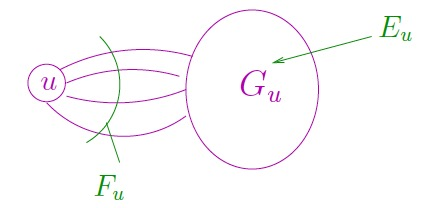
\includegraphics[width=0.4\textwidth]{vertexcover1.jpg}
\caption{Vertex Cover Substructure Lemma}\label{vertexcoverfigure}
\end{figure}
Since $S$ contains at least one endpoint for any edge in $E_u$, $S\cup\{u\}$ is a vertex cover of $G$ of size $k$.

($\Rightarrow$)
Let $S$ be a vertex cover of $G$ of size $k$. For any edge $(u,v)$, at least one of $u,v$ is inside $S$. Suppose $u\in S$. For any edge in $E_u$, at least one of its endpoints is in $S$, and it cannot be $u$, thus $S-\{u\}$ is a vertex cover of $G_u$ of size $k-1$.
\end{proof}
According to the substructure lemma, we can compute the vertex cover of a graph with Algorithm \ref{vertexcover}.
\begin{algorithm}[ht]
\caption{Vertex Cover Problem}\label{vertexcover}
\begin{algorithmic}[1]
\Input{Undirected graph $G=(V,E)$.}
\Output{Vertex cover of $G$ of size $k$.}
\If{$k=0$}
\If{$V=\emptyset$}
\State{Return $\emptyset$}
\Else\State{Fail}
\EndIf\EndIf
\State{Pick an arbitrary edge $(u,v)\in E$.}
\State{Recursively search for a vertex cover $S$ of size $k-1$ in $G_u$.}
\State{If found, return $S\cup\{u\}$.}
\State{Recursively search for a vertex cover $S$ of size $k-1$ in $G_v$.}
\State{If found, return $S\cup\{v\}$.}
\State{Fail.}\Comment{$G$ has no vertex cover of size $k$.}
\end{algorithmic}
\end{algorithm}

There are at most $O(2^k)$ recursive calls, each call takes $O(m)$ time (construction of $G_u$ or $G_v$), thus the overall running time is $O(m2^k)$, which is much better than $O(mn^k)$.

\subsection{Traveling Salesman Problem}
A brute-force search algorithm takes $O(n!)$ time. We will try to devise an algorithm with better running time. 

For every destination $j\in\{1,2,\dots,n\}$ and every subset $S\subseteq\{1,2,\dots,n\}$ that contains 1 and $j$, let $L_{S,j}$ represent the minimum length of a path from 1 to $j$ that visits each vertex in $S$ exactly once.
\begin{lemma}\textbf{Optimal Substructure Lemma}
Let $P$ be a shortest path from 1 to $j$ that visits each vertex in $S$ exactly once. If the last hop of $P$ is $(k,j)$ and the rest of $P$ is $P'$, then $P'$ is a shortest path from 1 to $k$ that visits each vertex in $S-\{j\}$ exactly once. 
\end{lemma}
The proof of the optimal substructure lemma is straightforward. According to the lemma, we have the induction relation
$$L_{S,j}=\min_{k\in S,k\neq j}\{L_{S-\{j\},k}+c_{kj}\}.$$
Algorithm \ref{tsp} is the dynamic programming algorithm based on this relation.
\begin{algorithm}[ht]
\caption{TSP Problem}\label{tsp}
\begin{algorithmic}[1]
\Input{A completed undirected graph with cost $c_{uv}$ for edge $(u,v)$.}
\Output{$2^n\times n$ 2D array $A$ with $A[S][j]=L_{S,j}$.}
\State{Initialize $A[S][1]=\begin{cases}
0&if\:S=\{1\}\\
+\infty&otherwise
\end{cases}$}
\For{$m=2,3,\dots,n$}\Comment{$m$ = subproblem size}
\For{each $S\subseteq\{1,2,\dots,n\}$ with $\lvert S\rvert=m$ and $1\in S$}
\For{each $j\in S$ and $j\neq 1$}
\State{$A[S][j]=\min_{k\in S,k\neq j}\{A[S-\{j\}][k]+c_{kj}\}$}
\EndFor\EndFor\EndFor
\State{Return $\min_{j=2,\dots,n}{A[\{1,2,\dots,n\}][j]+c_{j1}}$}
\end{algorithmic}
\end{algorithm}

There are $n2^n$ subproblems, each of which takes $O(n)$ time. Thus the overall running time is $O(n^22^n)$.

\section{Heuristics for NP-Complete Problems}
In this section we will use Knapsack problem as an example to illustrate the use of heuristics to tackle NP-complete problems.
\subsection{Greedy Heuristic}
In the Knapsack problem, we aim at maximize the total value of items under limited budget of total weight. Thus, ideal items are those with big value and small weight. A natural greedy choice is to always select the item with the largest $\frac{v}{w}$ ratio. However, this greedy approach has no guarantee of proximity to the optimal solution at all. For the simple example with $v_1=1,w_1=1,v_2=999,w_2=1000,W=1000$, we will end up with result 1, while the optimal is actually 999. 

A simple modification to this greedy heuristic can provide a fairly good proximity guarantee, as shown in Algorithm \ref{knapsackgreedyheuristic}.
\begin{algorithm}[ht]
\caption{Refined Greedy Heuristic for Knapsack Problem}\label{knapsackgreedyheuristic}
\begin{algorithmic}[1]
\Input{$n$ items with value $v_i$ and weight $w_i$ for item $i$. Total weight budget $W$(Assume that $w_i\leq W,\forall i$).}
\Output{A subset $S$ of the items that maximizes $\sum_{i\in S} v_i$ and subject to $\sum_{i\in S}w_i\leq W$.}
\State{Re-index the items so that $\frac{v_1}{w_1}\geq\frac{v_2}{w_2}\geq\dots\geq\frac{v_n}{w_n}$.}
\State{Put the items into $S'$ in order until one does not fit.}
\State{Let $k$ be the item with largest value.}
\If{$\sum_{i\in S'}v_i>v_k$}
\State{$S=S'$}
\Else\State{$S=\{k\}$.}
\EndIf
\end{algorithmic}
\end{algorithm}

The value of the solution provided by Algorithm \ref{knapsackgreedyheuristic} is always $\geq 50\%$ of the value of the optimal solution.
\begin{proof}
Suppose $S$ contains $m$ items, and we are allowed to put a fraction of item $m+1$ into $S$ so that $\sum_{i\in S}w_i=W$. Call this solution the ``greedy fractional solution''. Obviously this solution is at least as good as the optimal solution: it uses up the weight budget and guarantees larger overall $\frac{v}{w}$ ratio. 

Now let's consider the result of Algorithm \ref{knapsackgreedyheuristic}. It guarantees two conditions: 
\begin{align*}
\sum_{i\in S}v_i&\geq\sum_{i\in S'}v_i,\\
\sum_{i\in S}v_i&\geq v_k\geq v_{m+1}.
\end{align*}
Summing up the two inequalities, we have 
\begin{align*}
2\sum_{i\in S}v_i&\geq\sum_{i\in S'}v_i+v_{m+1}\\
&\geq\text{value of greedy fractional solution}\\
&\geq\text{value of optimal solution}\\
\end{align*}
Hence the value of the heuristic solution is at least 50\% of the value of the optimal solution.
\end{proof}
The 50\% proximity guarantee is tight, i.e. it is mathematically impossible to universally prove a better guarantee. Consider an example with $v_1=102,w_1=101,v_2=v_3=100,w_2=w_3=100$ and $W=200$. The optimal value is 200, while the solution provided by the refined greedy heuristic has value 102. 

Nonetheless, for specific inputs, the guarantee can be better. If $w_i\leq\delta W,\forall i$, in which $\delta$ is a small value such as 10\%, $S'$ is sure to use at least $(1-\delta)$ of $W$, thus value of the heuristic solution is at least $(1-\delta)$ of that of the optimal solution.
\subsection{DP Heuristic}
A dynamic programming heuristic can provide arbitrary proximity guarantee specified by user, making it possible to tune the trade-off between accuracy and running time. However this is not universal for all NP-complete problems.

In the last chapter we introduced a DP algorithm that solves the Knapsack problem in $O(nW)$ time. The subproblems were to calculate the maximal total value with total weight smaller than $x$ using only the first $i$ items, in which $i=0,1,\dots,n$ and $x=0,1,\dots,W$. There is actually another DP algorithm that solves another set of subproblems: for $i=0,1,\dots,n$ and $x=0,1,\dots,nv_{max}$, calculate the minimum total weight $S_{i,x}$ needed to achieve total value $\geq x$ using the first $i$ items. The recurrence relation is
\begin{equation*}
S_{i,x} = \min\{S_{i-1,x}, w_i+S_{i-1,x-v_i}\}
\end{equation*} 
$S_{i-1,x-v_i}$ is interpreted as 0 if $v_i>x$. The algorithm is shown in Algorithm \ref{knapsackdp2}. The overall algorithm is $O(n^2v_max)$.
\begin{algorithm}[ht]
\caption{Another DP Algorithm for Knapsack}\label{knapsackdp2}
\begin{algorithmic}[1]
\Input{$n$ items with value $v_i$ and weight $w_i$ for item $i$. Total weight budget $W$(Assume that $w_i\leq W,\forall i$).}
\Output{$n\times(nv_{max}+1)$ 2D array $A$ with $A[i][x]=S_{i,x}$.}
\State{Base case: $A[0][0]=0$, $A[0][x]=+\infty$ for $x\neq 0$.}
\For{$i=1,2,\dots,n$}
\For{$x=0,1,\dots,nv_{max}$}
\If{$v_i<x$}
\State{$A[i][x]=\min\{A[i-1][x],A[i-1][x-v_i]+w_i\}$}
\Else{$A[i][x]=\min\{A[i-1][x],w_i\}$}
\EndIf\EndFor\EndFor
\State{Return largest $x$ such that $A[n][x]\leq W$.}
\end{algorithmic}
\end{algorithm}

Algorithm \ref{knapsackdp2} requires that all $v_i$'s are integers. If they are small (polynomial in $n$), then the algorithm is already polynomial time. If that is not the case, a heuristic comes to our rescue. Its key idea is to solve a slightly incorrect but easier Knapsack instance in polynomial time. Specifically, we set $\hat{v_i}=\lfloor\frac{v_i}{m}\rfloor$ for each item and solve the Knapsack instance using $\hat{v_i}$'s as values. Now let's analyze its accuracy and running time.

Since $\frac{v_i}{m}-1<\lfloor\frac{v_i}{m}\rfloor\leq \frac{v_i}{m}$, we have $v_i-m<m\hat{v_i}\leq v_i$. Let $S$ represent the heuristic solution and $S^*$ represent the optimal solutions. Then we have $\sum_{i\in S}\hat{v_i}\geq \sum_{i\in S^*}\hat{v_i}$ because $S$ is optimal for $\hat{v_i}$'s. Therefore,
\begin{equation}\label{npknapsackeq1}
\sum_{i\in S}v_i\geq m\sum_{i\in S}\hat{v_i}\geq m\sum_{i\in S^*}\hat{v_i}> \sum_{i\in S^*}(v_i-m)\geq \sum_{i\in S^*}v_i-mn.
\end{equation}
In order to achieve $(1-\epsilon)$ proximity, we need to guarantee 
\begin{equation}\label{npknapsackeq2}
\sum_{i\in S^*}v_i-\sum_{i\in S}v_i\leq\epsilon\sum_{i\in S^*}v_i.
\end{equation}
According to \eqref{npknapsackeq1}, a sufficient condition for \eqref{npknapsackeq2} is  
\begin{equation*}
mn\leq \epsilon\sum_{i\in S^*}v_i,
\end{equation*}
which can be satisfied by setting
\begin{equation*}
m=\frac{\epsilon v_{max}}{n}.
\end{equation*}
In terms of running time, since $\hat{v_{max}}\leq\frac{v_{max}}{m}=\frac{n}{\epsilon}$, the overall running time is $O(n^2\hat{v_{max}}=O(n^3/\epsilon)$.

In summary, in order to guarantee $(1-\epsilon)$ proximity to the optimal solution, we should solve the Knapsack instance using $\hat{v_i}=\lfloor\frac{nv_i}{\epsilon v_{max}}\rfloor$ as value, and the running time will be $O(n^3/\epsilon)$.
\section{Local Search}
\subsection{Principles of Local Search}
In this section we will introduce a widely used paradigm to address NP complete problems: local search. 

Let $X$ be a set of solutions to a problem, for example all cuts of a graph, all possible tours of a TSP problem, all possible variable assignments of a constraint satisfaction problem, etc. For each $x\in X$, specify a subset of $X$ as its neighbors. For a graph cut, its neighborhood can be defined as the set of all cuts obtained by switching the side of one vertex; for a TSP tour, each neighbor differ from itself by 2 edges; for a CSP assignment, its neighbors differ from itself in the value of one single variable; etc. A general local search algorithm has the following structure:
\begin{enumerate}
\item Let $x$ be some solution.
\item While $x$ has a neighbor $y$ superior to itself, set $x\coloneqq y$.
\item Return the locally optimal solution $x$.
\end{enumerate}

There can be multiple local optimal solutions of a problems. If $X$ is finite and each iteration is guaranteed to improve some objective function, then the local search algorithm is guaranteed to terminate and converge to one of the local optimal solutions. However, it usually does not converge quickly. Neither is it guaranteed to provide a good approximation to the global optimal solution. To mitigate this shortcoming, we can run the local search multiple times with randomly chosen starting point, and return the best local optimal solution found. Different definition of neighborhood result in different local optimal solutions. In general bigger neighborhoods leads to fewer local optimal solutions, but makes it more difficult to verify local optimality, which is a quality-speed trade-off worthy of some tuning.
\subsection{Maximum Cut Problem}
\begin{description}
\Input{An undirected graph $G(V,E)$.}
\Output{A cut $(A,B)$ that maximizes the number of crossing edges.}
\end{description}
If the graph is a bipartite graph, the problem is solvable within linear time via BFS. Just start from any vertex and mark vertices reachable from it with odd number of steps with 1 and the rest with 0, then we obtain the maximum cut. However, in general this is an NP complete problem. We will introduce a local search algorithm that solves the problem.

For any cut $(A,B)$ and a vertex $v$, define 
\begin{description}
\item[$c_v(A,B)$]number of edges incident on $v$ that crosses $(A,B)$.
\item[$d_v(A,B)$]number of edges incident on $v$ that do not cross $(A,B)$.
\end{description}
Then we have the local search algorithm shown in Algorithm \ref{maxcutlocalsearch}.

\begin{algorithm}[ht]
\caption{Local Search of Maximum Cut}\label{maxcutlocalsearch}
\begin{algorithmic}[1]
\State{Let $(A,B)$ be an arbitrary cut of $G$.}
\While{there is a vertex $v$ with $d_v(A,B)>c_v(A,B)$}
\State{Move $v$ to the other side of the cut.}
\EndWhile
\State{Return the final cut $(A,B)$.}
\end{algorithmic}
\end{algorithm}
For graphs containing no parallel edges, the algorithm terminates within $\binom{n}{2}$ iterations because there are at most $\binom{n}{2}$ edges, and the number of crossing edges always increase by at least 1 before the algorithm converges. Hence the algorithm completes in polynomial time. 

In the output cut, we have $d_v(A,B)\leq c_v(A,B),\forall v\in V$. Hence 
\begin{align*}
\sum_vd_v(A,B)\leq \sum_vc_v(A,B).
\end{align*}
The lhs counts each non-crossing edge twice, while the rhs counts each crossing edge twice, thus 
\begin{align*}
2\cdot(\text{num of non-crossing edge})&\leq 2\cdot(\text{num of crossing edge})\\
&=2\cdot(\lvert E\rvert-\text{num of crossing edge})
\end{align*}
As a result, we have 
$$\text{num of non-crossing edge}\leq\frac{1}{2}\lvert E\rvert,$$ i.e. Algorithm \ref{maxcutlocalsearch} outputs a cut in which the number of crossing edges is at least $\frac{1}{2}\lvert E\rvert$, which is not at all an impressive performance guarantee because a the expectation of the number of crossing edges of a random cut is already $\frac{1}{2}\lvert E\rvert$.

In a more general case, each $e\in E$ has a non-negative weight $w_e$, and the aim of the problem becomes to maximize the total weight of the crossing edges. The local search algorithm is still well defined, and there is a similar 50\% performance guarantee. However, the algorithm is no longer guaranteed to converge in polynomial time, because the number of crossing edges is no longer guaranteed to increase in each iteration. The number of iterations can be exponential.
\subsection{The 2SAT Problem}
\begin{description}
\Input{$n$ boolean variables $x_i,i=1,2,\dots,n$. $m$ clauses of 2 literals each.}
\Output{Whether there exists an assignment to all $x_i$ that simultaneously satisfies all clauses.}
\end{description}
One example of the clauses with $n=m=4$ is $(x_1\lor x_2)\land(\neg x_1\lor x_3)\land(x_3\lor x_4)\land(\neg x_2\lor\neg x_4)$.

The 2SAT problem is a special case of the CSP that can be solved in polynomial time\footnote{It can be reduced to computing SCCs.}. 3SAT is on the contrary NP complete. We will analyze a random local search algorithm that solves the 2SAT problem, as shown in Algorithm \ref{twosatlocalsearch}.
\begin{algorithm}[ht]
\caption{Paradimitriou's Local Search 2SAT Algorithm}\label{twosatlocalsearch}
\begin{algorithmic}[1]
\For{$i=1$ \textbf{to} $\log n$}
\State{Choose a random initial assignment.}
\For{$j=1$ \textbf{to} $2n^2$}
\If{current assignment satisfies all clauses}
\State{Return this assignment}
\Else\State{Pick an arbitrary unsatisfied clause and flip the value of one of its two variables.}
\EndIf\EndFor\EndFor
\State{Report non-existence of such an assignment.}
\end{algorithmic}
\end{algorithm}
Obviously the algorithm runs in polynomial time and is always correct when there exists no satisfactory assignment. Nonetheless its performance guarantee is not trivial when such assignment exists.

To analyze Paradimitriou's algorithm, we need to first consider the problem of random walks on non-negative integers. Starting at 0, the position goes up or down by 1 at each step with 50/50 probability, except when the current position is 0, in which case we can only go to 1 with 100\% probability. Let $T_n$ represent the number of steps until the random walk reaches position $n$. 
\begin{theorem}
$E(T_n)=n^2$
\end{theorem}
\begin{proof}
Let $Z_i$ represent the number of steps needed to get from $i$ to $n$. Then we have
\begin{align*}
E(Z_n)&=0\\
E(Z_0)&=E(Z_1)+1\\
E(Z_i)&=\frac{1}{2}E(Z_{i+1})+\frac{1}{2}E(Z_{i-1})+1,\forall i\geq 1
\end{align*}
Therefore we have
\begin{equation*}
E(Z_i)-E(Z_{i+1})=E(Z_{i-1})-E(Z_i)+2,\forall i\geq 1,
\end{equation*}
which leads to 
\begin{align*}
E(Z_i)-E(Z_{i+1})=2i+1,\forall i\geq 0\\
\end{align*}
As a result,
\begin{align*}
E(Z_0)-E(Z_n)=\sum\limits_{i=0}^{n-1}\left(E(Z_i)-E(Z_{i+1})\right)=n^2.
\end{align*}
Hence $E(T^n)=E(Z_0)=n^2.$
\end{proof}
\begin{corollary}\label{localsearchcorollary}
$P\left(T_n>2n^2\right)<\frac{1}{2}$
\end{corollary}
\begin{proof}
\begin{align*}
n^2=E(T^n)&=\sum\limits_{i=0}^{2n^2}iP(T_n=i)+\sum\limits_{i=2n^2+1}^{\infty}iP(T_n=i)\\
&\geq\sum\limits_{i=2n^2+1}^{\infty}iP(T_n=i)\\
&>2n^2P\left(T_n>2n^2\right)\\
\end{align*}
Hence $P\left(T_n>2n^2\right)<\frac{1}{2}.$
\end{proof}
Now we can prove the following performance guarantee of Paradimitriou's local search algorithm.
\begin{theorem}
For a satisfiable 2SAT instance with $n$ variables, Paradimitriou's algorithm produces a satisfying assignment with probability $\geq 1-\frac{1}{n}$.
\end{theorem}
\begin{proof}
Let's focus on one iteration of the outer loop. 

Let $a^*$ represent an arbitrary satisfying assignment (there can be multiple such assignments), and let $a_t$ represent the assignment after $t$ iterations of the inner loop ($t=1,2,\dots,2n^2$). Let $\chi_t$ represent the number of variables on whose value $a^*$ and $a_t$ agree, thus $\chi_t$ is between 0 and $n$. 

If $\chi_t\neq n$, then there must be at least one unsatisfied clause. Suppose the clause concerns $x_i$ and $x_j$. The consequence of flipping the value of $x_i$ \textbf{or} $x_j$ (choose randomly) is:
\begin{itemize}
\item If $a^*$ and $a_t$ disagree on both $x_i$ and $x_j$: $\chi_{t+1}=\chi_t+1$.
\item If $a^*$ and $a_t$ disagree on one of $x_i$ and $x_j$:
\begin{equation*}
\chi_{t+1}=\begin{cases}
\chi_t+1&(50\%\:possibility)\\
\chi_t-1&(50\%\:possibility)\\
\end{cases}
\end{equation*}
\end{itemize}
There is an obvious analogy between the behavior of $\chi_t$ and the position in the random walks problem except:
\begin{enumerate}
\item Sometimes $\chi_t$ increases by 1 with possibility 100\%;
\item The process may terminate before $\chi_t=n$ because there could be other viable assignment;
\item Usually we start with $\chi_1>0$ instead of $\chi_1=0$: the miserable situation in which we start with the exact opposite of a satisfying assignment is rare. 
\end{enumerate}
All three differences only make it easier for the process to terminate correctly. Let $T$ represent the number of iterations needed inside each inner loop. According to Corollary \ref{localsearchcorollary}, we have $P(T>2n^2)<\frac{1}{2}$. Thus the probability that one iteration of the outer loop ends up with a satisfying assignment is at least $\frac{1}{2}$. With $\log n$ iterations, the probability that we end up with a correct solution is $\geq\frac{1}{2^{\log n}}=\frac{1}{n}.$


\end{proof}
\ifx\PREAMBLE\undefined
\end{document}
\fi